\documentclass[xcolor=dvipsnames,12pt]{beamer}

\usepackage[utf8x]{inputenc}
\usepackage[russian]{babel}
\usepackage[light,condensed,math]{iwona}
\usepackage[T1]{fontenc}

\usetheme{Rochester}
\usecolortheme[named=NavyBlue]{structure}

\begin{document}

\title{Санкт-Петербургский Политехнический Университет}
\date{}

\begin{frame}[plain] 
\titlepage
\end{frame}

\begin{frame}{Санкт-Петербургский Политехнический Университет}
Историю и славу Политехнического университета в течение более ста лет создавали люди, которые в нем преподавали и учились. Лауреаты Нобелевской премии П.Л. Капица, Н.Н. Семенов, Ж.И. Алферов, академики А.Ф. Иоффе, И.В. Курчатов, А.А. Радциг, Ю.Б. Харитон, ген. конструктор О.К. Антонов — это лишь несколько имен в ряду сотен талантливых ученых и организаторов производства, чья деятельность связана с Политехническим институтом и чьи достижения определили становление и развитие отечественной науки и техники.
\end{frame}

\begin{frame}{Санкт-Петербургский Политехнический Университет}

\begin{center}
\fbox{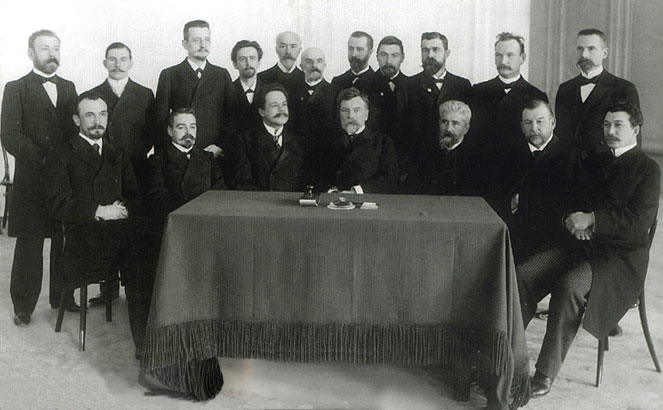
\includegraphics[width=5cm]{img1.jpg}}
\end{center}

На Псковской земле, в 15 км от древнего города Порхова, основанного новгородцами ещё в тринадцатом веке при князе Александре Невском, есть замечательное место Холомки. Здесь, в 1913 году первый ректор Политехнического, князь Андрей Григорьевич Гагарин построил усадебный дом. 
\end{frame}

\begin{frame}{Санкт-Петербургский Политехнический Университет}
В 2000 году в соответствии с распоряжением Комитета по управлению имуществом Псковской области, усадьба князя А.Г. Гагарина в Холомках была передана в постоянное владение Санкт-Петербургскому политехническому университету. С 2004 года университет ведет реставрацию усадьбы, которая стала учебно-историческим заповедником.
\end{frame}

\begin{frame}{Санкт-Петербургский Политехнический Университет}

\begin{center}
\fbox{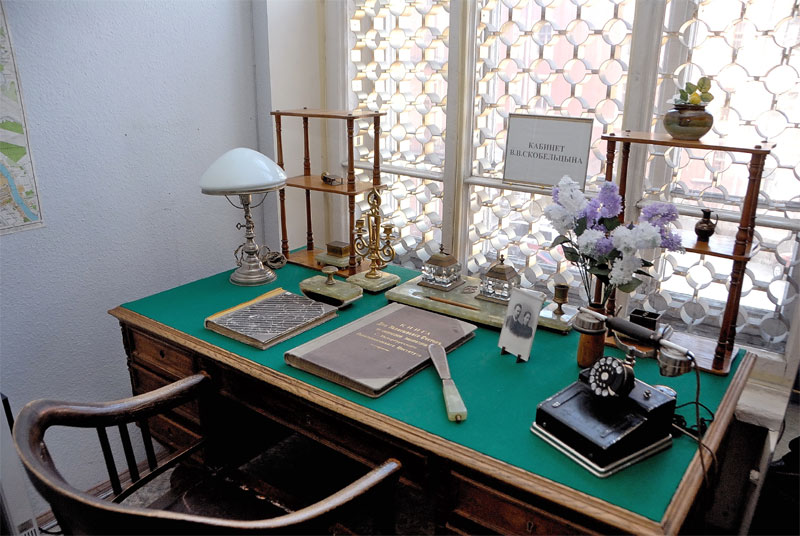
\includegraphics[width=5cm]{img2.jpg}}
\end{center}

Историко-технический музей Политехнического - один из крупнейших ВУЗовских музеев такого профиля, он хранит свыше 45000 экспонатов только основного фонда, в которых имеются машины и приборы конца ХIХ - начала ХХ века, модели, уникальные объекты техники и технологии.
\end{frame}

\begin{frame}{Санкт-Петербургский Политехнический Университет}
 Музей располагает материалами о важнейших событиях в жизни вуза. Старейшими из них являются фотодокументы, отснятые профессором Б.Н. Меншуткиным в период закладки и строительства института. Широко представлены в нем и материалы, отражающие вклад политехников в развитие науки и техники, в повышение обороноспособности страны. Движению студенческих строительных отрядов института посвящен отдельный раздел экспозиции, в котором - награды, полученные стройотрядами и зерно первого целинного урожая, привезенного студентами-политехниками в 1957 г.
\end{frame}
\end{document}